\chapter{अर्धसूत्री विभाजन, आनुवंशिक मिश्रण और वंशागति}\label{ch:b2:meiosis-heredity}

भूरी आँखों वाले दो माता-पिता की संतान नीली आँखों वाली होती है और किसी को
अचरज नहीं होता; एक ही माता-पिता के दो बच्चे कभी एक जैसे नहीं होते, और
इस पर भी किसी को अचरज नहीं होता। दोनों तथ्य एक ही प्रक्रिया से निकलते
हैं। हर अंडाणु और हर शुक्राणु बनते समय, हर गुणसूत्र की दो प्रतियों वाली
कोई कोशिका ठीक एक प्रति आगे सौंपती है, यादृच्छिक रूप से चुनी हुई, और वह
भी दोनों प्रतियों को खंड बदलने देने के बाद। फिर हर निषेचन ऐसे दो
अर्ध-समुच्चय जोड़ देता है जो कभी मिले ही नहीं थे। यह अध्याय उसी
प्रक्रिया का --- \omterm{def:b2:meiosis-heredity:meiosis}{अर्धसूत्री विभाजन} का --- वर्णन करता है, और उन
वंशागति-नियमों का जो उससे निकलते हैं: मेंडेल के अनुपात, उनके अपवाद, एक
ही गुणसूत्र साझा करते जीनों की \omterm{def:b2:meiosis-heredity:linkage}{सहलग्नता} और उससे बनने वाले मानचित्र, तथा
\omterm{prop:b2:meiosis-heredity:sexlinked}{लिंग गुणसूत्रों} और कोशिकांगों की अनोखी वंशागति।

\section{अर्धसूत्री विभाजन}

\begin{definition}[अर्धसूत्री विभाजन]\label{def:b2:meiosis-heredity:meiosis}
\index{अर्धसूत्री विभाजन}\index{अगुणित}\index{द्विगुणित}
कोई \emph{द्विगुणित} कोशिका ($2n$) हर प्रकार के दो \emph{समजात}
गुणसूत्र ढोती है, हर जनक से एक, जो जीन-अंतर्वस्तु में एक जैसे हैं पर
युग्मविकल्पियों में ज़रूरी नहीं। \emph{अर्धसूत्री विभाजन} विभाजनों की
वह जोड़ी है जो एक द्विगुणित कोशिका को चार \emph{अगुणित} कोशिकाओं ($n$)
में बदल देती है, जिनमें से हर एक में हर प्रकार का एक गुणसूत्र होता है।
उससे पहले एक प्रतिकृतिकरण होता है, इसलिए हर गुणसूत्र दो सहोदरी
क्रोमैटिडों के रूप में प्रवेश करता है; पहला विभाजन \emph{समजातों} को
अलग करता है (न्यूनकारी), दूसरा \emph{सहोदरी क्रोमैटिडों} को
(समकारी), जैसा समसूत्री विभाजन करता है। प्राणियों में अर्धसूत्री विभाजन
युग्मक बनाता है; पौधों और कवकों में बीजाणु (\cref{ch:b2:plant-life-cycles});
और हर लैंगिक जीव में यही वह पग है जो गुणसूत्र-संख्या आधी करता है ताकि
निषेचन उसे फिर दुगुना कर सके।
\end{definition}

\begin{proposition}[अवस्थाएँ]\label{prop:b2:meiosis-heredity:stages}
\index{पूर्वावस्था I}\index{सूत्रयुग्मन}\index{काएज़्मा}\index{जीन-विनिमय}
\emph{\omterm{prop:b2:meiosis-heredity:stages}{पूर्वावस्था I}} लंबी है और मिश्रण यहीं होता है।
प्रतिकृत गुणसूत्र संघनित होते हैं; हर एक अपना समजात ढूँढ़ता है और उससे
जीन-दर-जीन युग्मित होता है (\emph{सूत्रयुग्मन}), और उन्हें प्रोटीन की
एक सीढ़ी, \emph{सूत्रयुग्मी संकुल}, थामे रहती है, जिससे चार क्रोमैटिडों
का एक \emph{द्विसंयोजी} बनता है; असहोदरी क्रोमैटिड मेल खाते बिंदुओं पर
टूटते और फिर जुड़ते हैं (\emph{जीन-विनिमय}), प्रति द्विसंयोजी एक से कई
बार; और जब वह संकुल घुल जाता है, तब समजात केवल इन्हीं विनिमय-बिंदुओं पर
जुड़े रह जाते हैं, जो \emph{काएज़्मा} के रूप में दिखते हैं।
\emph{मध्यावस्था I}: द्विसंयोजी तर्कु पर पंक्तिबद्ध होते हैं, और हर
जोड़ी यादृच्छिक रूप से अभिविन्यस्त होती है --- मातृ समजात एक ध्रुव की
ओर या दूसरे की, हर दूसरी जोड़ी से स्वतंत्र। \emph{पश्चावस्था I}:
समजात अलग होते हैं और सहोदरी क्रोमैटिड साथ रहती हैं; हर ध्रुव को दो-दो
क्रोमैटिड वाले $n$ गुणसूत्र मिलते हैं। \emph{अंत्यावस्था I}
और, प्रायः बिना प्रतिकृतिकरण के, \emph{\omterm{def:b2:meiosis-heredity:meiosis}{अर्धसूत्री विभाजन} II}: वे $n$
गुणसूत्र अकेले-अकेले पंक्तिबद्ध होते हैं, सहोदरी क्रोमैटिड अलग होती
हैं, और चार \omterm{def:b2:meiosis-heredity:meiosis}{अगुणित} केंद्रक बनते हैं। \omterm{def:b2:meiosis-heredity:meiosis}{अर्धसूत्री विभाजन} I में घंटों
से दशकों तक लगते हैं (कोई मानव अंडाणुक जन्म से पहले से लेकर अंडोत्सर्ग
तक \omterm{prop:b2:meiosis-heredity:stages}{पूर्वावस्था I} में ठहरा रहता है);
\omterm{def:b2:meiosis-heredity:meiosis}{अर्धसूत्री विभाजन} II में एक घंटा लगता है।
\end{proposition}

\begin{omfigure}
\begin{tikzpicture}[every node/.style={font=\scriptsize}]
  % helper: cell outline at (x,y)
  \foreach \x/\lab in {0/{पूर्वावस्था I: युग्मन, जीन-विनिमय}, 3.2/{मध्यावस्था I: द्विसंयोजी पंक्तिबद्ध}, 6.4/{पश्चावस्था I: समजात अलग होते हैं}, 9.6/{अर्धसूत्री विभाजन II: क्रोमैटिड अलग होती हैं}}
    { \draw[thick] (\x+1.2,0) circle (1.15); \node[below, align=center, text width=2.8cm] at (\x+1.2,-1.2) {\lab}; }
  % prophase I: one bivalent with chiasma
  \draw[very thick, omDef] (0.8,-0.5) -- (0.8,0.5); \draw[very thick, omDef] (1.0,-0.5) -- (1.0,0.5);
  \draw[very thick, omThm] (1.4,-0.5) -- (1.4,0.5); \draw[very thick, omThm] (1.6,-0.5) -- (1.6,0.5);
  \draw[very thick, omDef] (1.0,0.1) -- (1.4,-0.1); \draw[very thick, omThm] (1.4,0.1) -- (1.0,-0.1);
  \fill[white] (0.9,-0.03) rectangle (1.5,0.03);
  \draw[very thick, omDef] (1.0,0.1) -- (1.4,-0.1); \draw[very thick, omThm] (1.4,0.1) -- (1.0,-0.1);
  \node[omExo!60!black] at (1.2,-0.85) {काएज़्मा};
  % metaphase I: two bivalents on the plate, spindle
  \begin{scope}[xshift=3.2cm]
    \draw[gray, dashed] (1.2,-1.0) -- (1.2,1.0);
    \foreach \y in {0.45,-0.45} {
      \draw[very thick, omDef] (0.95,\y-0.25) -- (0.95,\y+0.25); \draw[very thick, omDef] (1.08,\y-0.25) -- (1.08,\y+0.25);
      \draw[very thick, omThm] (1.32,\y-0.25) -- (1.32,\y+0.25); \draw[very thick, omThm] (1.45,\y-0.25) -- (1.45,\y+0.25);
    }
    \draw[gray] (0.15,0) -- (0.95,0.45); \draw[gray] (0.15,0) -- (0.95,-0.45);
    \draw[gray] (2.25,0) -- (1.45,0.45); \draw[gray] (2.25,0) -- (1.45,-0.45);
  \end{scope}
  % anaphase I
  \begin{scope}[xshift=6.4cm]
    \foreach \y in {0.45,-0.45} {
      \draw[very thick, omDef] (0.45,\y-0.25) -- (0.45,\y+0.25); \draw[very thick, omDef] (0.58,\y-0.25) -- (0.58,\y+0.25);
      \draw[very thick, omThm] (1.82,\y-0.25) -- (1.82,\y+0.25); \draw[very thick, omThm] (1.95,\y-0.25) -- (1.95,\y+0.25);
    }
    \draw[->, gray] (1.2,0) -- (0.75,0); \draw[->, gray] (1.2,0) -- (1.65,0);
  \end{scope}
  % meiosis II: four cells
  \begin{scope}[xshift=9.6cm]
    \foreach \p/\c in {(0.75,0.5)/omDef,(1.65,0.5)/omDef,(0.75,-0.5)/omThm,(1.65,-0.5)/omThm} {
      \draw[thick, gray!60] \p circle (0.38);
      \draw[very thick, \c] \p ++(-0.12,-0.2) -- ++(0,0.4);
      \draw[very thick, \c] \p ++(0.12,-0.2) -- ++(0,0.4);
    }
  \end{scope}
\end{tikzpicture}

{\small समजातों की दो जोड़ियों के लिए \omterm{def:b2:meiosis-heredity:meiosis}{अर्धसूत्री विभाजन} (मातृ नीले,
पितृ लाल, हर एक दो क्रोमैटिडों का)। समजात \omterm{prop:b2:meiosis-heredity:stages}{पूर्वावस्था I} में युग्मित
होते और खंड बदलते हैं, मध्यावस्था I में द्विसंयोजी के रूप में पंक्तिबद्ध
होते हैं, पश्चावस्था I में अलग होते हैं; और \omterm{def:b2:meiosis-heredity:meiosis}{अर्धसूत्री विभाजन} II
क्रोमैटिडों को चार \omterm{def:b2:meiosis-heredity:meiosis}{अगुणित} कोशिकाओं में बाँट देता है।}
\end{omfigure}

\begin{omfigure}
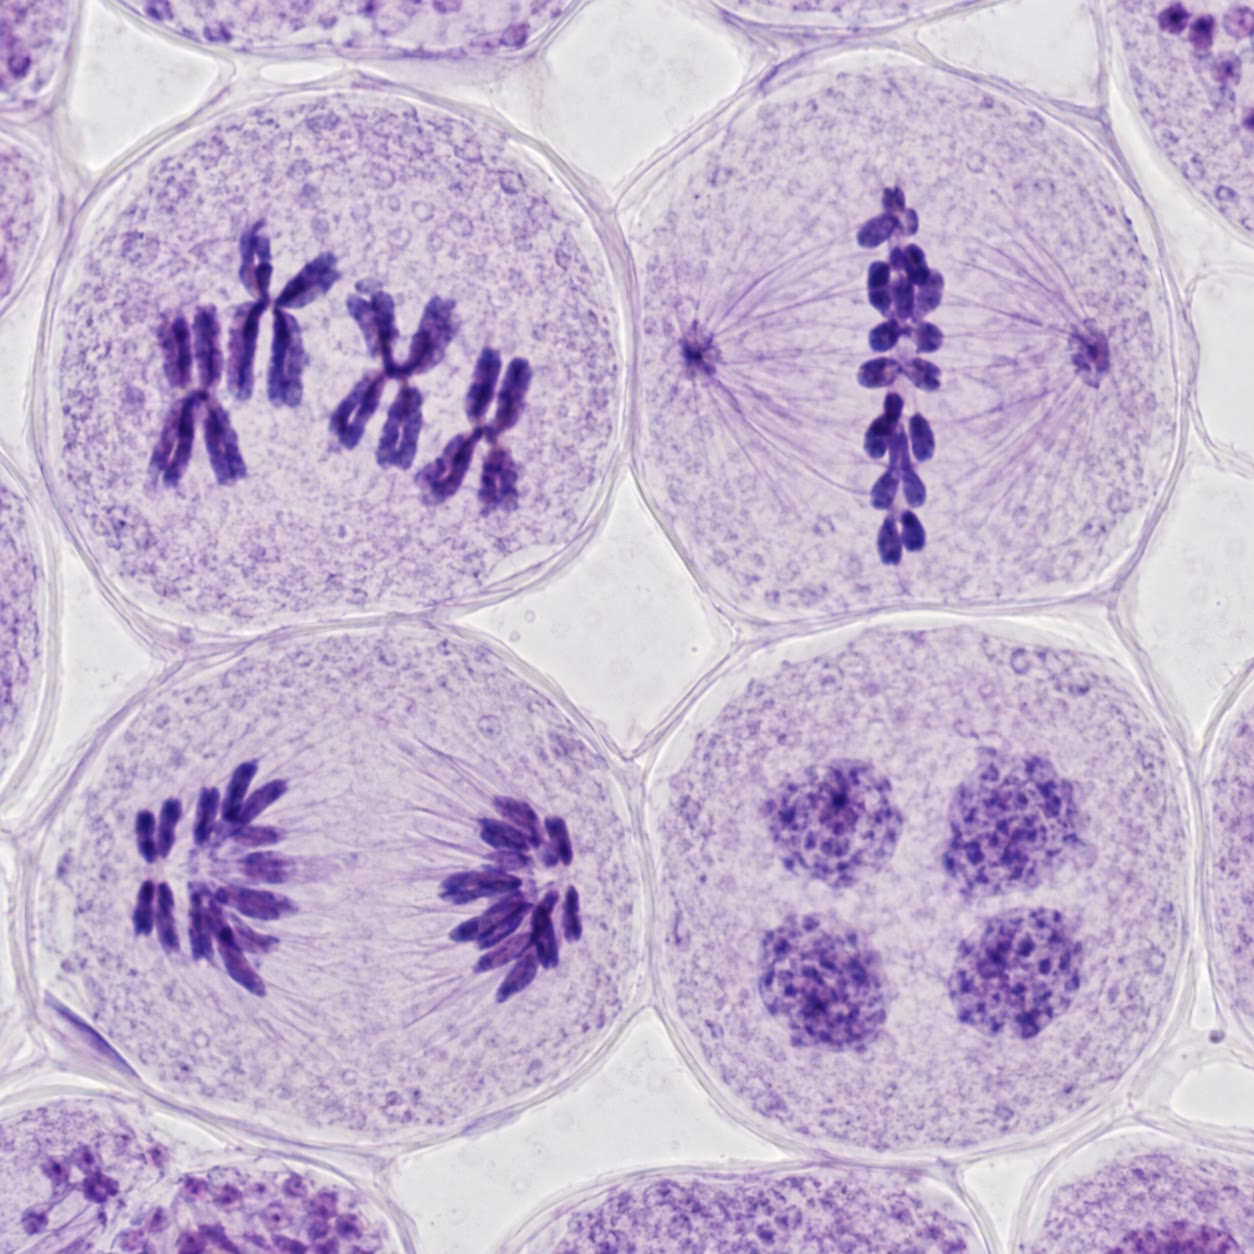
\includegraphics[width=0.5\linewidth]{images/book4/ai/b4-04-lily-meiosis.jpg}

{\small किसी लिली के परागकोश में \omterm{def:b2:meiosis-heredity:meiosis}{अर्धसूत्री विभाजन}: पिछली \omterm{prop:b2:meiosis-heredity:stages}{पूर्वावस्था
I} के द्विसंयोजी, एक मध्यावस्था I पट्ट, पश्चावस्था I, और किसी चतुष्क के चार केंद्रक।}
\end{omfigure}

\begin{theorem}[अर्धसूत्री विभाजन कितना मिश्रण करता है]\label{thm:b2:meiosis-heredity:mixing}
\index{स्वतंत्र अपव्यूहन}\index{आनुवंशिक पुनर्संयोजन}
गुणसूत्रों की $n$ जोड़ियों वाले किसी जीव में मध्यावस्था I पर
द्विसंयोजियों का यादृच्छिक अभिविन्यास किसी युग्मक में मातृ और पितृ
गुणसूत्रों के $2^n$ संभव संयोजन बनाता है ---
मनुष्य में $2^{23} \approx 8.4$ लाख --- और किसी युग्मनज में
$2^{2n}$। जीन-विनिमय इसे और गुणा कर देता है: प्रति द्विसंयोजी लगभग $k$
काएज़्मा, और हर एक की स्थिति बदलती हुई, तो भिन्न युग्मकों की संख्या
व्यावहारिक रूप से असीम है, और किसी एक व्यक्ति के दो युग्मक कभी एक जैसे
नहीं होते। \emph{पुनर्संयोजन} --- युग्मविकल्पियों के नए संयोजन ---
दोनों से उठता है: \omterm{thm:b2:meiosis-heredity:mixing}{स्वतंत्र अपव्यूहन} पूरे गुणसूत्र फिर से फेंटता है,
जीन-विनिमय किसी एक गुणसूत्र के भीतर के जीन।
\end{theorem}
\begin{proof}
हर द्विसंयोजी दो परिणामों के साथ स्वतंत्र रूप से अभिविन्यस्त होता है,
इसलिए $n$ द्विसंयोजी $2^n$ संयोजन देते हैं, और सब समसंभाव्य। दोनों
जनकों में से हर एक ऐसा एक युग्मक देता है, इसलिए युग्मनज के पास $2^n\times
2^n$ हैं। $L$ क्षारक युग्मों के किसी गुणसूत्र में किसी भिन्न स्थिति पर
हुआ जीन-विनिमय प्रति द्विसंयोजी $L$ की कोटि की भिन्न पुनर्संयोजी
क्रोमैटिड दे सकता है, इसलिए भिन्न उत्पादों की गिनती प्रति गुणसूत्र $L^k$
की तरह बढ़ती है, जो $L \sim 10^8$ के लिए खगोलीय है।
\end{proof}
\begin{proof}[प्रमाण-सामग्री]
क्राइटन और मक्लिंटॉक (1931) ने मक्का का ऐसा गुणसूत्र 9 काम में लिया जो
दो दृश्य कोशिकावैज्ञानिक चिह्न (एक सिरे पर एक गाँठ, दूसरे पर एक
स्थानांतरित खंड) और उनके बीच दो जीन (रंगीन/रंगहीन दाना, मोमी/मंडीय
भ्रूणपोष) ढोता था। संतति में हर वह पौधा जिसमें युग्मविकल्पियों की जोड़ी
पुनर्संयोजित थी, उसमें कोशिकावैज्ञानिक चिह्नों की जोड़ी भी पुनर्संयोजित
थी --- गाँठ बिना स्थानांतरण के या उलटा --- और इससे सिद्ध हुआ कि
\omterm{thm:b2:meiosis-heredity:mixing}{आनुवंशिक पुनर्संयोजन} गुणसूत्र-खंडों का भौतिक विनिमय है।
\end{proof}

\begin{omfigure}
\begin{tikzpicture}[every node/.style={font=\scriptsize}]
  \foreach \dx/\lab/\ca/\cb/\gam in {0/{अभिविन्यास 1}/omDef/omThm/{युग्मक AB और ab}, 6.2/{अभिविन्यास 2}/omThm/omDef/{युग्मक Ab और aB}} {
    \begin{scope}[xshift=\dx cm]
      \draw[gray, dashed] (0,-1.1) -- (3.2,-1.1);
      \node[anchor=south] at (1.6,0.6) {\lab};
      % pair 1 (long): A above the plate, a below
      \draw[very thick, omDef] (0.7,-0.95) -- (0.7,-0.25); \node[omDef, anchor=south] at (0.7,-0.2) {A};
      \draw[very thick, omThm] (0.7,-1.25) -- (0.7,-1.95); \node[omThm, anchor=north] at (0.7,-2.0) {a};
      % pair 2 (short): B or b above depending on orientation
      \draw[very thick, \ca] (2.3,-0.85) -- (2.3,-0.35);
      \draw[very thick, \cb] (2.3,-1.35) -- (2.3,-1.85);
      \node[anchor=north] at (1.6,-2.4) {\gam};
    \end{scope}
  }
  \node[omDef, anchor=south] at (2.3,-0.3) {B}; \node[omThm, anchor=north] at (2.3,-1.9) {b};
  \node[omThm, anchor=south] at (8.5,-0.3) {b}; \node[omDef, anchor=north] at (8.5,-1.9) {B};
  \node[anchor=north, align=center] at (4.7,-3.0) {हर अभिविन्यास समान रूप से संभाव्य:\\युग्मक AB, ab, Ab, aB बराबर संख्या में --- स्वतंत्र अपव्यूहन};
\end{tikzpicture}

{\small \omterm{thm:b2:meiosis-heredity:mixing}{स्वतंत्र अपव्यूहन}। गुणसूत्रों की दो जोड़ियों (एक पर A/a,
दूसरी पर B/b) के लिए मध्यावस्था I पर द्विसंयोजियों के दोनों संभव
अभिविन्यास समान रूप से संभाव्य हैं, इसलिए युग्मकों में चारों
\omterm{def:b2:meiosis-heredity:vocabulary}{युग्मविकल्पी} संयोजन बराबर संख्या में दिखते हैं।}
\end{omfigure}

\section{मेंडेली विश्लेषण}

\begin{definition}[संकरणों की शब्दावली]\label{def:b2:meiosis-heredity:vocabulary}
\index{युग्मविकल्पी}\index{जीन-प्ररूप}\index{लक्षण-प्ररूप}\index{प्रभावी}\index{अप्रभावी}\index{समयुग्मजी}\index{विषमयुग्मजी}
कोई \emph{जीन} गुणसूत्र का एक टुकड़ा है; उसके \emph{युग्मविकल्पी} उसके
अनुक्रम-विभेद हैं; और \emph{स्थल} उसकी स्थिति है। कोई \omterm{def:b2:meiosis-heredity:meiosis}{द्विगुणित}
व्यक्ति हर स्थल पर दो युग्मविकल्पी ढोता है: उसका \emph{जीन-प्ररूप}
\emph{समयुग्मजी} ($AA$, $aa$) या \emph{विषमयुग्मजी} ($Aa$) होता है।
\emph{लक्षण-प्ररूप} वह लक्षण है जो दिखता है। कोई युग्मविकल्पी
\emph{प्रभावी} है जब विषमयुग्मजी उसका लक्षण-प्ररूप दिखाए, और
\emph{अप्रभावी} जब वह केवल समयुग्मजी में दिखे; यह भेद युग्मविकल्पियों
की जोड़ी का और देखे जाते लक्षण का गुण है, अकेले युग्मविकल्पी का नहीं ---
अधिकांश अप्रभावी युग्मविकल्पी कार्य-लोप के युग्मविकल्पी हैं, जो इसलिए
छिपे रहते हैं कि एक काम करती प्रति पर्याप्त है। कोई \emph{शुद्ध वंशक्रम}
सत्य-प्रजनन करता है (समयुग्मजी); कोई \emph{परीक्षण संकरण} प्रभावी
लक्षण-प्ररूप वाले किसी व्यक्ति का संगम किसी अप्रभावी समयुग्मजी से कराता
है, ताकि उसकी संतति उसके युग्मकों के युग्मविकल्पी सीधे उजागर कर दे।
\end{definition}

\begin{theorem}[मेंडेल के अनुपात]\label{thm:b2:meiosis-heredity:mendel}
\index{मेंडेल के नियम}\index{एकसंकर संकरण}\index{द्विसंकर संकरण}
चूँकि किसी \omterm{def:b2:meiosis-heredity:vocabulary}{विषमयुग्मजी} $Aa$ के दोनों \omterm{def:b2:meiosis-heredity:vocabulary}{युग्मविकल्पी} बराबर संख्या में
भिन्न युग्मकों में पृथक होते हैं (पश्चावस्था I), इसलिए कोई
\emph{एकसंकर} संकरण $Aa \times Aa$ \omterm{def:b2:meiosis-heredity:vocabulary}{जीन-प्ररूप} $\tfrac14 AA : \tfrac12 Aa :
\tfrac14 aa$ देता है, और \omterm{def:b2:meiosis-heredity:vocabulary}{लक्षण-प्ररूप} $3 : 1$ यदि $A$ \omterm{def:b2:meiosis-heredity:vocabulary}{प्रभावी} हो; और
परीक्षण संकरण $Aa \times aa$ $1 : 1$ देता है। चूँकि भिन्न गुणसूत्रों के
जीनों के \omterm{def:b2:meiosis-heredity:vocabulary}{युग्मविकल्पी} स्वतंत्र रूप से अपव्यूहित होते हैं (मध्यावस्था I),
इसलिए कोई \emph{द्विसंकर} $AaBb$ चार प्रकार के युग्मक बराबर संख्या में
बनाता है और संकरण $AaBb \times AaBb$ \omterm{def:b2:meiosis-heredity:vocabulary}{लक्षण-प्ररूप} $9 : 3 : 3 : 1$ देता
है, तथा परीक्षण संकरण $AaBb \times aabb$ $1 : 1 : 1 : 1$। $k$ स्वतंत्र
\omterm{def:b2:meiosis-heredity:vocabulary}{विषमयुग्मजी} स्थलों के लिए युग्मक-प्रकारों की संख्या $2^k$ है और
लक्षण-प्ररूपी अनुपात $k$ अनुपातों $3 : 1$ का गुणनफल।
\end{theorem}
\begin{proof}
पृथक्करण: \omterm{def:b2:meiosis-heredity:vocabulary}{विषमयुग्मजी} के युग्मक $\tfrac12 A$,
$\tfrac12 a$ हैं; और यादृच्छिक निषेचन के साथ युग्मनज के \omterm{def:b2:meiosis-heredity:vocabulary}{जीन-प्ररूप}
गुणनफल $(\tfrac12 A + \tfrac12 a)^2 = \tfrac14 AA + \tfrac12 Aa +
\tfrac14 aa$ हैं। स्वतंत्रता: $AaBb$ के युग्मक $(\tfrac12 A
+ \tfrac12 a)(\tfrac12 B + \tfrac12 b)$ हैं, यानी $\tfrac14$ पर चार
प्रकार; और द्विसंकर \omterm{def:b2:meiosis-heredity:vocabulary}{लक्षण-प्ररूप} $(\tfrac34 A\_ + \tfrac14 aa)
(\tfrac34 B\_ + \tfrac14 bb)$ का गुणनफल हैं, यानी $\tfrac{9}{16}, \tfrac{3}{16},
\tfrac{3}{16}, \tfrac{1}{16}$। हर गुणक एक स्वतंत्र पृथक्करण है,
इसलिए $k$ स्थल $k$ गुणकों का गुणनफल देते हैं।
\end{proof}
\begin{proof}[प्रमाण-सामग्री]
मेंडेल (1866) ने मटर के शुद्ध वंशक्रमों का संकरण कराया जो एक-एक लक्षण
में भिन्न थे --- गोल या झुर्रीदार बीज, पीला या हरा बीजपत्र, बैंगनी या
सफ़ेद फूल, लंबा या बौना तना और तीन और --- और हर बार पहली पीढ़ी एकरूप
पाई तथा दूसरी पीढ़ी $3 : 1$ के पास पृथक होती हुई: 5474 गोल बनाम 1850
झुर्रीदार ($2.96 :
1$), 6022 पीले बनाम 2001 हरे ($3.01 : 1$), 705 बैंगनी बनाम 224 सफ़ेद
($3.15 : 1$)। दो-लक्षण संकरणों में उन्हें $315 : 108 : 101 :
32$ ($9 : 3 : 3 : 1$) मिला, और दूसरी पीढ़ी को आगे उगाकर उन्होंने
दिखाया कि \omterm{def:b2:meiosis-heredity:vocabulary}{प्रभावी} वर्ग दो प्रकार का है, एक तिहाई शुद्ध और दो तिहाई
पृथक होता हुआ। जो गुणसूत्र इन अनुपातों को समझाते हैं वे चालीस वर्ष बाद
मिले।
\end{proof}

\begin{omfigure}
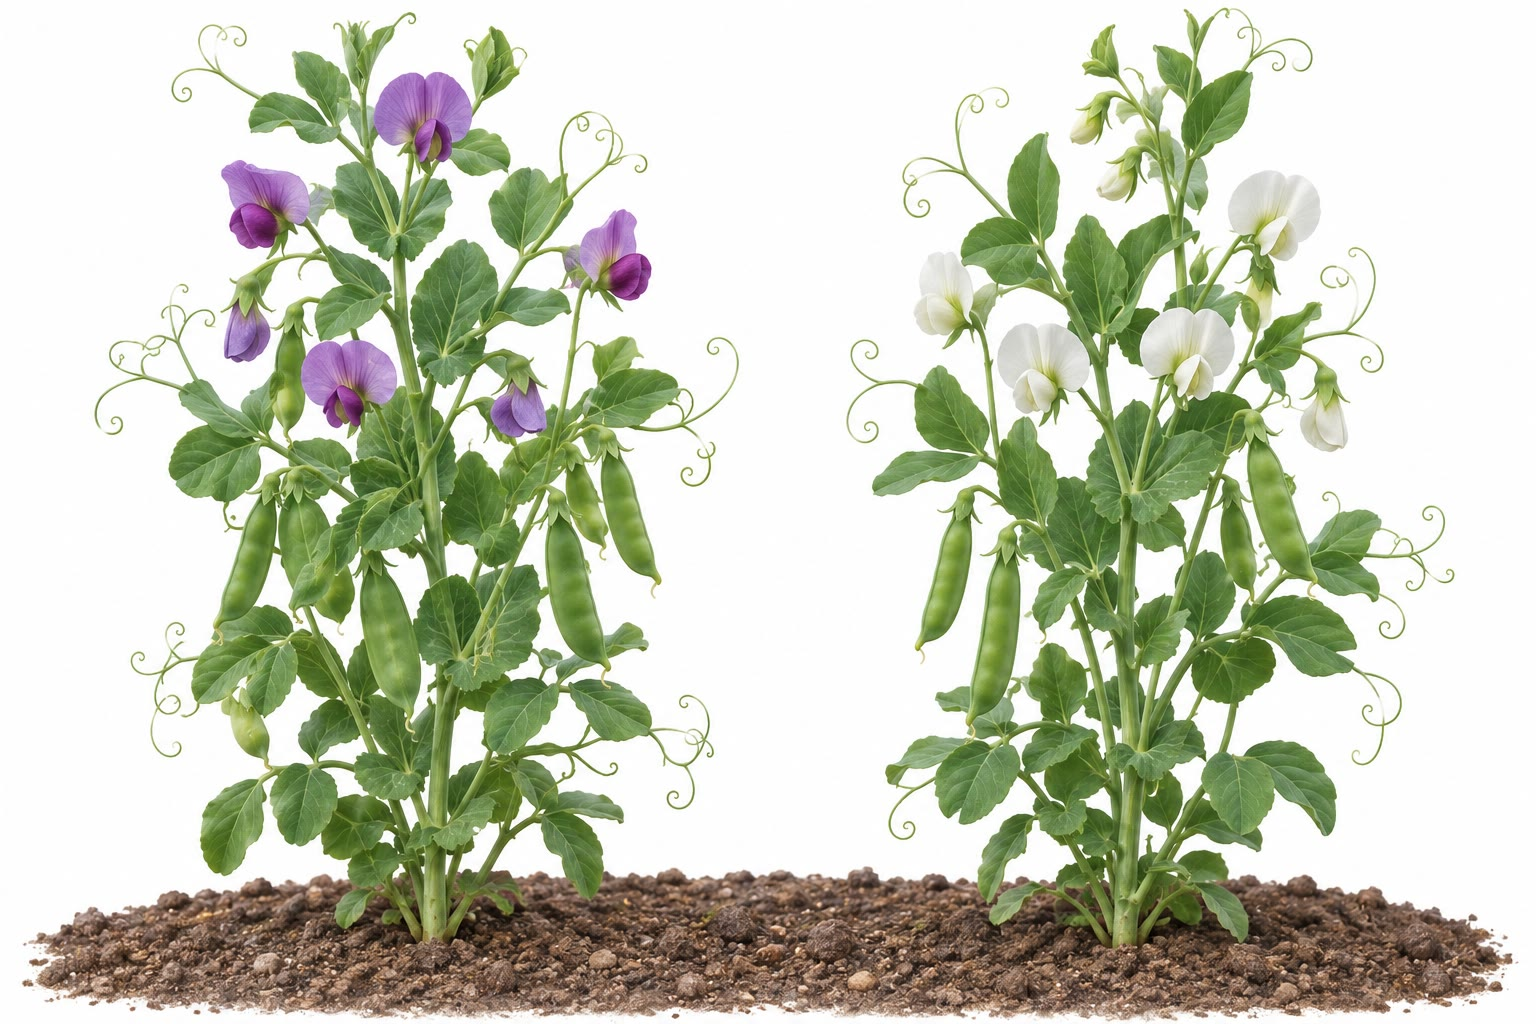
\includegraphics[width=0.58\linewidth]{images/book4/ai/b4-04-pea-flowers.jpg}

{\small बैंगनी फूलों वाले और सफ़ेद फूलों वाले मटर के पौधे: उन सात
लक्षण-जोड़ियों में से एक जिन पर मेंडेल ने आनुवंशिकी की नींव रखी। बैंगनी
फूलों वाला संकर स्वपरागित हो तो लगभग तीन बैंगनी बनाम एक सफ़ेद देता है।}
\end{omfigure}

\begin{method}[किसी अनुपात को $\chi^2$ से परखना]\label{met:b2:meiosis-heredity:chisquare}
\index{काई-वर्ग परीक्षण}
यह तय करने के लिए कि प्रेक्षित गिनतियाँ $O_i$ किसी परिकल्पित अनुपात पर बैठती हैं या नहीं:
\begin{enumerate}
  \item उस अनुपात और कुल से प्रत्याशित गिनतियाँ $E_i$ निकालिए।
  \item $\chi^2 = \sum_i (O_i - E_i)^2/E_i$ निकालिए।
  \item स्वातंत्र्य कोटियाँ गिनिए: वर्गों की संख्या घटा एक।
  \item \qty{5}{\%} स्तर पर क्रांतिक मान से तुलना कीजिए:
        1 स्वातंत्र्य कोटि के लिए $3.84$, 2 के लिए $5.99$, 3 के लिए $7.81$,
        4 के लिए $9.49$। यदि $\chi^2$ उससे नीचे हो तो आँकड़े उस अनुपात
        के अनुरूप हैं; यदि ऊपर हो तो अनुपात अस्वीकृत है --- वह विचलन
        बीस में एक से भी कम प्रयोगों में संयोग से उठता।
\end{enumerate}
मेंडेल के फूलों के लिए, $705 : 224$ बनाम $3 : 1$: $E = 696.75,
232.25$; $\chi^2 = 0.098 + 0.293 = 0.39 < 3.84$। (इन क्रांतिक मानों के
पीछे का बंटन गणित शृंखला के सांख्यिकी भाग में व्युत्पन्न है; यहाँ यह
सारणी एक औज़ार भर है।)
\end{method}

\begin{proposition}[सरल अनुपातों से आगे]\label{prop:b2:meiosis-heredity:extensions}
\index{अपूर्ण प्रभाविता}\index{सहप्रभाविता}\index{एपिस्टैसिस}\index{घातक युग्मविकल्पी}
अनुपात बदलते हैं, पर क्रियाविधि नहीं, जब: \omterm{def:b2:meiosis-heredity:vocabulary}{युग्मविकल्पी}
\emph{\omterm{prop:b2:meiosis-heredity:extensions}{अपूर्ण प्रभाविता}} दिखाएँ (लाल $\times$ सफ़ेद स्नैपड्रैगन
गुलाबी देता है, और दूसरी पीढ़ी $1 : 2 : 1$); \omterm{def:b2:meiosis-heredity:vocabulary}{युग्मविकल्पी}
\emph{सहप्रभावी} हों और दोनों अभिव्यक्त हों ($AB$ रक्त: \omterm{def:b2:meiosis-heredity:vocabulary}{विषमयुग्मजी}
$I^AI^B$ दोनों प्रतिजन बनाता है; किसी स्थल पर \emph{बहु
\omterm{def:b2:meiosis-heredity:vocabulary}{युग्मविकल्पी}} हो सकते हैं, $I^A$, $I^B$, $i$); कोई \omterm{def:b2:meiosis-heredity:vocabulary}{युग्मविकल्पी}
\omterm{def:b2:meiosis-heredity:vocabulary}{समयुग्मजी} अवस्था में \emph{घातक} हो (पीले चूहे: पीला $\times$ पीला $2$ पीले
बनाम $1$ ऐगूटी देता है, और $\tfrac14 YY$ भ्रूण के रूप में मर जाते हैं);
दो जीन एक ही पथ में काम करें (\emph{एपिस्टैसिस}: किसी $9 : 3 : 3 : 1$
संकरण में दोहरा \omterm{def:b2:meiosis-heredity:vocabulary}{अप्रभावी} और कोई एकल \omterm{def:b2:meiosis-heredity:vocabulary}{अप्रभावी} एक-से दिख सकते हैं और
$9 : 3 : 4$ देते हैं, जैसा ऐल्बिनो चूहों में, या \omterm{def:b2:meiosis-heredity:vocabulary}{लक्षण-प्ररूप} के लिए
दोनों \omterm{def:b2:meiosis-heredity:vocabulary}{प्रभावी} चाहिए हो सकते हैं और $9 : 7$ मिलता है, जैसा उन बैंगनी
मीठे मटरों में जिन्हें अपना रंजक बनाने के लिए दो एंजाइम चाहिए); या अनेक
जीन किसी संतत लक्षण (ऊँचाई, उपज) में थोड़ा-थोड़ा जोड़ें, जो
\cref{ch:b2:population-genetics} की मात्रात्मक आनुवंशिकी है। किसी
अनुपात से पीछे किसी क्रियाविधि तक पढ़ना आनुवंशिकी का रोज़मर्रा का हुनर है।
\end{proposition}

\section{सहलग्नता और आनुवंशिक मानचित्र}

\begin{definition}[सहलग्नता और पुनर्संयोजन बारंबारता]\label{def:b2:meiosis-heredity:linkage}
\index{सहलग्नता}\index{पुनर्संयोजन बारंबारता}\index{सेंटीमॉर्गन}
एक ही गुणसूत्र के दो जीन \emph{सहलग्न} हैं: उनके \omterm{def:b2:meiosis-heredity:vocabulary}{युग्मविकल्पी}
साथ-साथ युग्मकों में जाने की ओर झुके रहते हैं, और कोई द्विसंकर
$AB/ab$ \emph{जनकीय} युग्मक ($AB$, $ab$) \emph{पुनर्संयोजी} युग्मकों
($Ab$, $aB$) से अधिक बनाता है। पुनर्संयोजी तभी उठते हैं जब दोनों स्थलों
के बीच कोई जीन-विनिमय पड़े, इसलिए उनकी बारंबारता $r$ --- जो किसी
परीक्षण संकरण में सीधे गिनी जाती है --- वही दूरी मापती है: $r$
0 (पूर्ण सहलग्नता) से $\tfrac12$ (इतने दूर के, या भिन्न गुणसूत्रों के,
जीन कि वे स्वतंत्र रूप से अपव्यूहित हों) तक फैलता है।
\emph{मानचित्र-दूरी} का मात्रक \emph{सेंटीमॉर्गन} (cM) है: \qty{1}{cM}
निकट सहलग्न जीनों के लिए \qty{1}{\%} पुनर्संयोजन है; मनुष्य में
\qty{1}{cM} लगभग दस लाख क्षारक युग्म है। सहलग्नता ही पहला प्रमाण थी कि
जीन गुणसूत्र पर एक पंक्ति में बैठे हैं।
\end{definition}
\begin{proof}[प्रमाण-सामग्री]
मॉर्गन (1911) ने पाया कि मक्खी के सफ़ेद-आँख और लघु-पंख जीन, जो दोनों
X गुणसूत्र पर हैं, स्वतंत्र रूप से अपव्यूहित नहीं होते: किसी
परीक्षण संकरण ने \qty{50}{\%} के बजाय \qty{37}{\%} पुनर्संयोजी दिए,
और दूसरी जोड़ियों ने दूसरे, पर दोहराए जा सकने वाले, प्रतिशत। स्टर्टेवेंट
(1913) ने, स्नातक छात्र रहते हुए, समझा कि यदि ये बारंबारताएँ दूरियाँ
मापती हैं तो उन्हें जुड़ना चाहिए: X-सहलग्न छह जीनों की जोड़ीवार
बारंबारताओं से उन्होंने पहला आनुवंशिक मानचित्र खींचा, और वे दूरियाँ,
त्रुटि के भीतर, एक रेखा पर योगशील थीं।
\end{proof}

\begin{omfigure}
\begin{tikzpicture}[every node/.style={font=\scriptsize}]
  % bivalent with crossover between A and B
  \draw[very thick, omDef] (0,1.2) -- (2.0,1.2) -- (3.0,0.6) -- (5,0.6);
  \draw[very thick, omDef] (0,1.5) -- (5,1.5);
  \draw[very thick, omThm] (0,0.3) -- (2.0,0.3) -- (3.0,0.9) -- (5,0.9);
  \draw[very thick, omThm] (0,0) -- (5,0);
  \node[omDef, above] at (0.8,1.5) {A}; \node[omDef, above] at (4.3,1.5) {B};
  \node[omThm, below] at (0.8,0) {a}; \node[omThm, below] at (4.3,0) {b};
  \node[anchor=south, gray] at (2.5,1.85) {A और B स्थलों के बीच जीन-विनिमय};
  % products
  \draw[->, thick, gray] (5.4,0.75) -- (6.2,0.75);
  \node[anchor=west, align=left] at (6.4,1.45) {\textcolor{omDef}{A\,B} \quad जनकीय};
  \node[anchor=west, align=left] at (6.4,0.95) {\textcolor{omDef}{A}\,\textcolor{omThm}{b} \quad पुनर्संयोजी};
  \node[anchor=west, align=left] at (6.4,0.5) {\textcolor{omThm}{a}\,\textcolor{omDef}{B} \quad पुनर्संयोजी};
  \node[anchor=west, align=left] at (6.4,0.0) {\textcolor{omThm}{a\,b} \quad जनकीय};
  \node[anchor=west, align=left, text width=5.6cm] at (6.4,-0.9) {अर्धसूत्री विभाजनों के किसी अंश $c$ में दोनों स्थलों के बीच एक जीन-विनिमय: पुनर्संयोजी युग्मक $r = c/2$, क्योंकि चार में से केवल दो क्रोमैटिड ही बदली जाती हैं};
\end{tikzpicture}

{\small दो सहलग्न स्थलों के बीच पुनर्संयोजन। किसी द्विसंयोजी में उनके
बीच हुआ जीन-विनिमय चार में से दो क्रोमैटिडों पर \omterm{def:b2:meiosis-heredity:vocabulary}{युग्मविकल्पी} बदल देता
है; पुनर्संयोजी युग्मक किसी परीक्षण संकरण में गिने जाते हैं, और उनकी
बारंबारता वह दूरी माप देती है।}
\end{omfigure}

\begin{method}[दो सहलग्न जीनों का मानचित्रण]\label{met:b2:meiosis-heredity:twopoint}
\begin{enumerate}
  \item द्विसंकर पाने के लिए दो शुद्ध वंशक्रमों का संकरण कराइए; ध्यान
        रखिए कि उसे कौन-से \omterm{def:b2:meiosis-heredity:vocabulary}{युग्मविकल्पी} साथ मिले (उसके जनकीय संयोजन,
        \emph{युग्मन} $AB/ab$ या \emph{विकर्षण} $Ab/aB$)।
  \item उसका परीक्षण संकरण दोहरे \omterm{def:b2:meiosis-heredity:vocabulary}{अप्रभावी} से कराइए और संतति का
        वर्गीकरण कीजिए: दो सबसे बड़े वर्ग जनकीय हैं, दो सबसे छोटे
        पुनर्संयोजी।
  \item $r = $ पुनर्संयोजी $/$ कुल; दूरी $100\,r$ cM है।
  \item पहले स्वतंत्रता जाँचिए: यदि चारों वर्ग बराबर हों
        ($\chi^2$ बनाम $1 : 1 : 1 : 1$), तो जीन असहलग्न हैं।
\end{enumerate}
\end{method}

\begin{theorem}[हैल्डेन का मानचित्रण फलन]\label{thm:b2:meiosis-heredity:haldane}
\index{मानचित्रण फलन}
दूर-दूर के जीनों के लिए \omterm{def:b2:meiosis-heredity:linkage}{पुनर्संयोजन बारंबारता} दूरी को कम आँकती है,
क्योंकि उनके बीच के दो जीन-विनिमय जनकीय संयोजन लौटा देते हैं। यदि
जीन-विनिमय गुणसूत्र पर स्वतंत्र रूप से पड़ें (कोई व्यतिकरण नहीं), और
$d$ मॉर्गन में मानचित्र-दूरी हो (प्रति क्रोमैटिड जीन-विनिमयों की
प्रत्याशित संख्या), तो पुनर्संयोजन अंश है
\[
r = \tfrac12\,\bigl(1 - e^{-2d}\bigr), \qquad d = -\tfrac12\ln(1 - 2r),
\]
इसलिए $r \approx d$ छोटे $d$ के लिए, और $r \to \tfrac12$ जब $d$ बढ़े;
$r = 0.40$ \qty{80}{cM} के संगत है, और \qty{50}{cM}
$r = 0.32$ देता है। असल गुणसूत्र \emph{व्यतिकरण} दिखाते हैं --- कोई
जीन-विनिमय पास के दूसरे को कम संभाव्य बना देता है --- जो छोटी दूरियों पर
$r$ को हैल्डेन की भविष्यवाणी से अधिक $d$ के पास ले आता है।
\end{theorem}
\begin{proof}
मान लीजिए मानचित्र-दूरी $d$ उस अंतराल में प्रति क्रोमैटिड जीन-विनिमयों
की प्रत्याशित संख्या है; चूँकि हर जीन-विनिमय में चार में से दो
क्रोमैटिड लगती हैं, इसलिए पूरा द्विसंयोजी उस अंतराल में $2d$ माध्य की
पॉइसों संख्या में जीन-विनिमय ढोता है, और उसके एक भी न ढोने की प्रायिकता
$e^{-2d}$ है। यदि वह कम से कम एक ढोए, तो हर जीन-विनिमय में
किसी दी हुई क्रोमैटिड के लगने की प्रायिकता स्वतंत्र रूप से
$\tfrac12$ है, इसलिए कोई दी हुई क्रोमैटिड विषम बार बदली गई है --- यानी
पुनर्संयोजी है --- और यह प्रायिकता ठीक $\tfrac12$ है, चाहे
जीन-विनिमयों की संख्या कुछ भी हो। इसलिए $r = \tfrac12\,(1 -
e^{-2d})$; और उलटने पर $d$ मिलता है। छोटे $d$ के लिए $r \approx d$;
$d \to \infty$ पर $r \to \tfrac12$।
\end{proof}

\begin{omfigure}
\begin{tikzpicture}
\begin{axis}[
  width=0.72\linewidth, height=5.6cm,
  axis x line=bottom, axis y line=left,
  xmin=0, xmax=150, ymin=0, ymax=0.55,
  xlabel={मानचित्र-दूरी $d$ (cM)}, ylabel={पुनर्संयोजन अंश $r$},
  xlabel style={font=\small, at={(axis description cs:0.5,-0.13)}, anchor=north},
  ylabel style={font=\small},
  tick label style={font=\small}, xtick={0,50,100,150}, ytick={0,0.25,0.5},
  legend style={font=\scriptsize, at={(0.97,0.1)}, anchor=south east, draw=none},
  clip=false,
]
\addplot[very thick, omDef, domain=0:150, samples=80] {0.5*(1-exp(-2*x/100))};
\addlegendentry{हैल्डेन: $r = \tfrac12(1 - e^{-2d})$}
\addplot[thick, dashed, gray, domain=0:50, samples=2] {x/100};
\addlegendentry{$r = d$ (कोई दोहरा जीन-विनिमय नहीं)}
\draw[dashed, gray] (axis cs:0,0.5) -- (axis cs:150,0.5);
\end{axis}
\end{tikzpicture}

{\small मानचित्र-दूरी के सापेक्ष पुनर्संयोजन अंश। पास-पास के जीन अपनी
दूरी के समानुपात में पुनर्संयोजित होते हैं; दूर के जीन चाहे जितने दूर
हों, \qty{50}{\%} पुनर्संयोजन से कभी आगे नहीं जाते, क्योंकि दोहरे
जीन-विनिमय जनकीय संयोजन लौटा देते हैं।}
\end{omfigure}

\begin{method}[त्रिबिंदु परीक्षण संकरण]\label{met:b2:meiosis-heredity:threepoint}
\index{त्रिबिंदु संकरण}\index{व्यतिकरण}
किसी त्रिगुण \omterm{def:b2:meiosis-heredity:vocabulary}{विषमयुग्मजी} $ABC/abc$ का संकरण $abc/abc$ से कराइए और
संतति के आठ वर्गों का वर्गीकरण कीजिए।
\begin{enumerate}
  \item दो सबसे बड़े वर्ग जनकीय हैं; दो सबसे छोटे \emph{दोहरे
        जीन-विनिमय} हैं।
  \item जो जीन किसी जनकीय वर्ग और दोहरे-जीन-विनिमय वर्ग के बीच बदलता
        है वही \emph{बीच} वाला है: इससे क्रम मिल जाता है।
  \item हर आसन्न जोड़ी के लिए \omterm{def:b2:meiosis-heredity:linkage}{पुनर्संयोजन बारंबारता}
        (उस अंतराल के एकल जीन-विनिमय + दोहरे जीन-विनिमय) $/$
        कुल है, क्योंकि कोई दोहरा जीन-विनिमय दोनों अंतराल पुनर्संयोजित
        कर देता है।
  \item प्रत्याशित दोहरे जीन-विनिमय $= r_1 r_2 \times$ कुल;
        \emph{संपात गुणांक} प्रेक्षित/प्रत्याशित है और
        \emph{व्यतिकरण} $1 -$ संपात।
\end{enumerate}
\end{method}

\begin{example}[एक त्रिबिंदु संकरण, हल किया हुआ]\label{ex:b2:meiosis-heredity:threepoint}
$+++/abc \times abc/abc$ की संतति: $+++$ 580, $abc$ 592, $++c$
45, $ab+$ 40, $+bc$ 89, $a++$ 94, $+b+$ 3, $a+c$ 5; कुल 1448।
जनकीय $+++$, $abc$; दोहरे $+b+$, $a+c$; $+++$ की तुलना
$+b+$ से करने पर जो जीन बदला वह $b$ है: क्रम $a$--$b$--$c$। $r_{ab} =
(89 + 94 + 3 + 5)/1448 = 0.132$; $r_{bc} = (45 + 40 + 3 + 5)/1448 =
0.064$; मानचित्र: $a$ --- \qty{13.2}{cM} --- $b$ --- \qty{6.4}{cM} ---
$c$। प्रत्याशित दोहरे $0.132\times 0.064\times 1448 = 12.2$,
प्रेक्षित 8: संपात $0.65$, व्यतिकरण $0.35$।
\end{example}

\begin{omfigure}
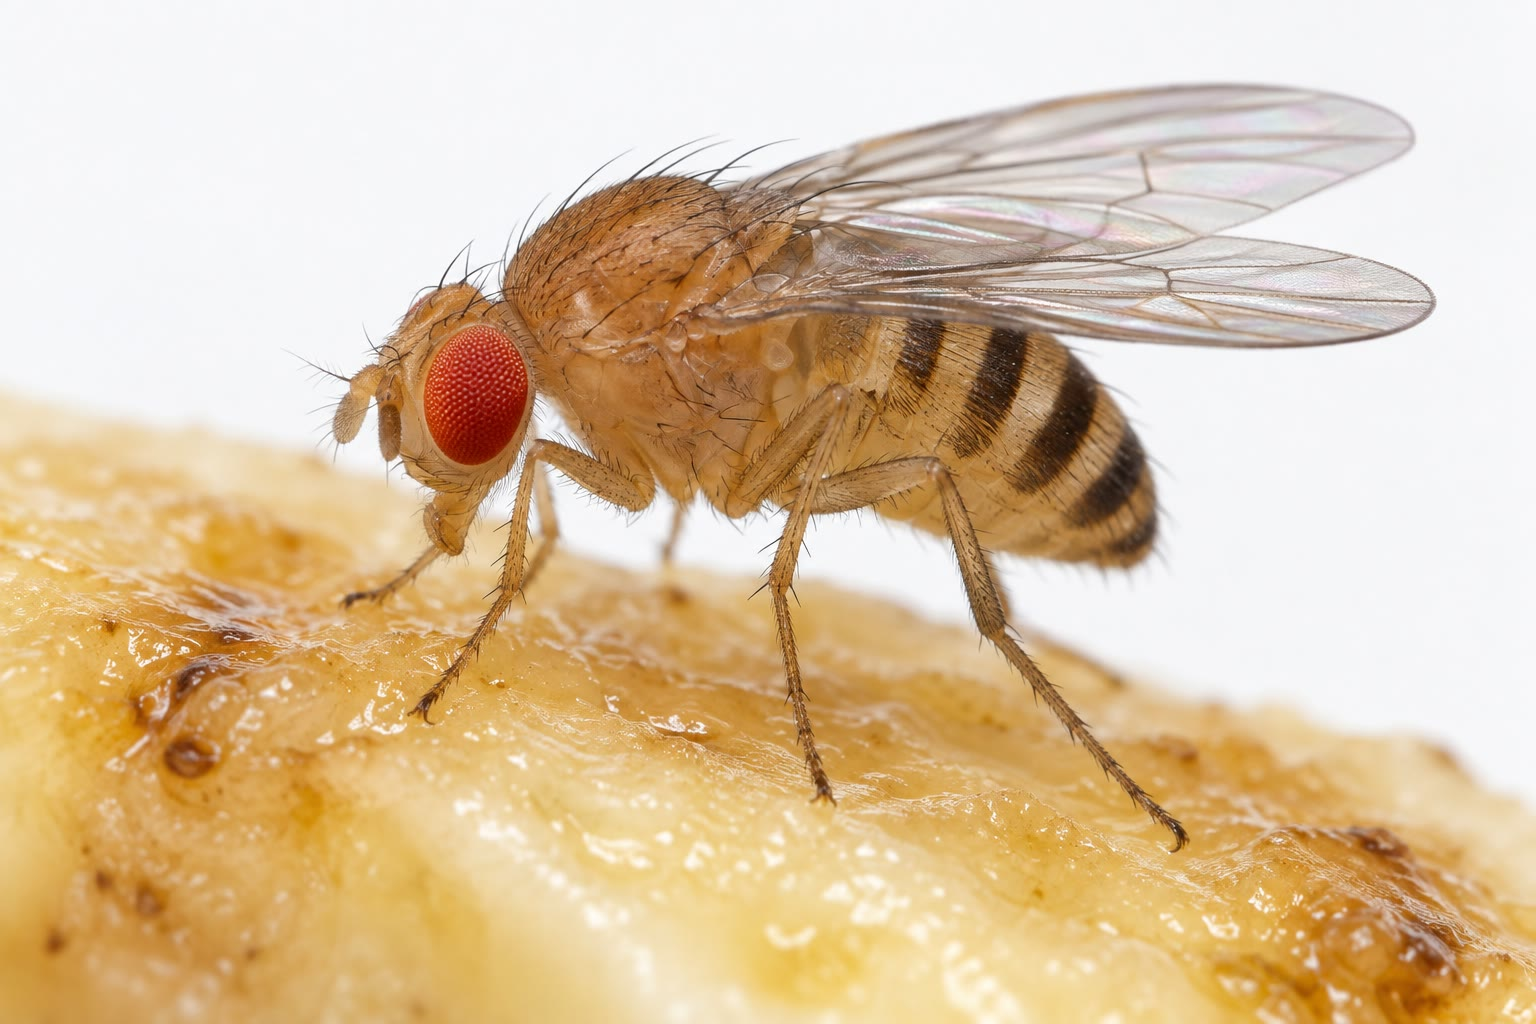
\includegraphics[width=0.5\linewidth]{images/book4/ai/b4-04-drosophila.jpg}

{\small \emph{Drosophila melanogaster}: प्रति पीढ़ी दो सप्ताह,
सैकड़ों संतान, गुणसूत्रों की चार जोड़ियाँ, और उत्परिवर्तियों की एक
शताब्दी --- वही जीव जिस पर \omterm{def:b2:meiosis-heredity:linkage}{सहलग्नता}, मानचित्र और लिंग-सहलग्न
वंशागति सुलझाई गई।}
\end{omfigure}

\section{लिंग गुणसूत्र और कोशिकांग}

\begin{proposition}[लिंग-सहलग्न वंशागति]\label{prop:b2:meiosis-heredity:sexlinked}
\index{X-सहलग्न वंशागति}\index{लिंग गुणसूत्र}
स्तनधारियों और मक्खियों में मादा $XX$ है और नर $XY$: $Y$ थोड़े ही जीन
ढोता है, इसलिए नर के पास हर $X$-सहलग्न जीन की एक ही प्रति होती है (वह
\emph{अर्धयुग्मजी} है) और वह जो भी \omterm{def:b2:meiosis-heredity:vocabulary}{युग्मविकल्पी} ढोए उसे दिखाता है,
\omterm{def:b2:meiosis-heredity:vocabulary}{प्रभावी} हो या \omterm{def:b2:meiosis-heredity:vocabulary}{अप्रभावी}। परिणाम: व्युत्क्रम संकरण भिन्न होते हैं
(सफ़ेद-आँख मादा $\times$ लाल-आँख नर सफ़ेद-आँख पुत्र और लाल-आँख पुत्रियाँ
देता है; उलटा संकरण सब लाल देता है); कोई \omterm{def:b2:meiosis-heredity:vocabulary}{अप्रभावी}
$X$-सहलग्न लक्षण (लाल--हरा वर्णांधता, हीमोफ़ीलिया, ड्यूशेन
पेशीय दुष्पोषण) अधिकतर नरों में दिखता है, अप्रभावित वाहक माताओं से आगे
बढ़ता है, और पिता से पुत्र को कभी नहीं जाता (पुत्र को पिता का $Y$ मिलता
है); और पिता अपना $X$ अपनी सारी पुत्रियों को देता है।
पक्षी, तितलियाँ और कुछ सरीसृप इस व्यवस्था को उलट देते हैं ($ZW$
मादाएँ, $ZZ$ नर); अनेक सरीसृप तापमान को निर्णय करने देते हैं; और
स्तनधारियों में हर मादा कोशिका का एक $X$ विकास में जल्दी ही यादृच्छिक
रूप से चुप करा दिया जाता है, इसलिए कोई \omterm{def:b2:meiosis-heredity:vocabulary}{विषमयुग्मजी} मादा एक मोज़ेक होती
है (कछुआ-रंग बिल्ली)।
\end{proposition}
\begin{proof}[प्रमाण-सामग्री]
मॉर्गन (1910) को हज़ारों लाल-आँख मक्खियों में एक सफ़ेद-आँख नर मिला। लाल
मादाओं से संकरण कराने पर सारी संतति लाल थी; पर अगली पीढ़ी में सफ़ेद
आँखें केवल नरों में, और उनमें भी आधों में, फिर दिखीं। किसी सफ़ेद नर का
संकरण उसी की लाल पुत्रियों से कराने पर दोनों लिंगों में सफ़ेद आँखें
मिलीं। यह प्रतिरूप ठीक वही था जो तब अपेक्षित है जब वह जीन X गुणसूत्र पर
बैठा हो, जिसे मादाएँ दो बार और नर एक बार ढोते हैं --- यानी किसी
गुणसूत्र को सौंपा गया पहला जीन।
\end{proof}

\begin{omfigure}
\begin{tikzpicture}[every node/.style={font=\scriptsize}]
  % pedigree: X-linked recessive
  \draw[thick, fill=gray!70] (0,0) rectangle (0.5,0.5); % affected grandfather
  \draw[thick] (1.5,0.25) circle (0.25);
  \draw[thick] (0.5,0.25) -- (1.25,0.25);
  \draw[thick] (0.875,0.25) -- (0.875,-0.5);
  \draw[thick] (0.875,-0.5) -- (3.5,-0.5);
  % children of generation I
  \draw[thick] (0.875,-0.5) -- (0.875,-0.9); \draw[thick, fill=white] (0.875,-1.15) circle (0.25); \fill (0.875,-1.15) circle (0.08);
  \draw[thick] (2.2,-0.5) -- (2.2,-0.9); \draw[thick] (1.95,-1.4) rectangle (2.45,-0.9);
  \draw[thick] (3.5,-0.5) -- (3.5,-0.9); \draw[thick, fill=white] (3.5,-1.15) circle (0.25); \fill (3.5,-1.15) circle (0.08);
  % carrier daughter marries
  \draw[thick] (-0.3,-1.15) -- (0.625,-1.15); \draw[thick] (-0.55,-1.4) rectangle (-0.05,-0.9);
  \draw[thick] (0.15,-1.15) -- (0.15,-1.9); \draw[thick] (-1.2,-1.9) -- (1.5,-1.9);
  \draw[thick] (-1.2,-1.9) -- (-1.2,-2.3); \draw[thick, fill=gray!70] (-1.45,-2.8) rectangle (-0.95,-2.3);
  \draw[thick] (-0.3,-1.9) -- (-0.3,-2.3); \draw[thick] (-0.55,-2.8) rectangle (-0.05,-2.3);
  \draw[thick] (0.6,-1.9) -- (0.6,-2.3); \draw[thick, fill=white] (0.6,-2.55) circle (0.25); \fill (0.6,-2.55) circle (0.08);
  \draw[thick] (1.5,-1.9) -- (1.5,-2.3); \draw[thick, fill=white] (1.5,-2.55) circle (0.25);
  \node[anchor=east] at (-1.8,0.25) {I};
  \node[anchor=east] at (-1.8,-1.15) {II};
  \node[anchor=east] at (-1.8,-2.55) {III};
  % legend
  \node[anchor=west, align=left] at (5,-0.4) {$\square$ नर \quad $\bigcirc$ मादा};
  \draw[thick, fill=gray!70] (5.05,-1.25) rectangle (5.45,-0.85); \node[anchor=west] at (5.6,-1.05) {प्रभावित};
  \draw[thick] (5.25,-1.85) circle (0.2); \fill (5.25,-1.85) circle (0.07); \node[anchor=west] at (5.6,-1.85) {वाहक (विषमयुग्मजी)};
  \node[anchor=north west, align=left, text width=6.2cm] at (5,-2.3) {X-सहलग्न अप्रभावी: किसी प्रभावित पुरुष की संतान अप्रभावित होती है, उसकी सारी पुत्रियाँ वह युग्मविकल्पी ढोती हैं, और उनके आधे पुत्र प्रभावित होते हैं --- लक्षण एक पीढ़ी छोड़ देता है और नातियों में फिर दिखता है};
\end{tikzpicture}

{\small हीमोफ़ीलिया जैसे किसी X-सहलग्न \omterm{def:b2:meiosis-heredity:vocabulary}{अप्रभावी} लक्षण की
वंशावली: पिता से पुत्र को संचरण नहीं, वाहक पुत्रियाँ, प्रभावित नाती।}
\end{omfigure}

\begin{method}[कोई वंशावली पढ़ना]\label{met:b2:meiosis-heredity:pedigree}
\index{वंशावली}
\begin{enumerate}
  \item दो अप्रभावित माता-पिता और एक प्रभावित संतान: लक्षण
        \omterm{def:b2:meiosis-heredity:vocabulary}{अप्रभावी} है (दोनों जनक \omterm{def:b2:meiosis-heredity:vocabulary}{विषमयुग्मजी})।
  \item किसी प्रभावित संतान का कोई जनक सदा प्रभावित हो, और लक्षण हर
        पीढ़ी में दिखे: \omterm{def:b2:meiosis-heredity:vocabulary}{प्रभावी}।
  \item प्रभावित व्यक्ति अधिकतर नर हों, संचरण अप्रभावित माताओं से हो,
        और पिता से पुत्र को कभी नहीं: X-सहलग्न \omterm{def:b2:meiosis-heredity:vocabulary}{अप्रभावी}।
  \item किसी प्रभावित पिता की सारी पुत्रियाँ प्रभावित हों और कोई पुत्र
        प्रभावित न हो: X-सहलग्न \omterm{def:b2:meiosis-heredity:vocabulary}{प्रभावी}।
  \item माताओं से उनकी सारी संतानों को संचरित हो, पिताओं से कभी नहीं:
        सूत्रकणिकीय।
  \item फिर निहित \omterm{def:b2:meiosis-heredity:vocabulary}{जीन-प्ररूपों} से प्रायिकताएँ निकालिए:
        किसी वाहक $\times$ सामान्य दंपती के हर जन्म पर किसी प्रभावित
        पुत्र की प्रायिकता $\tfrac14$ है ($\tfrac12$ लड़का $\times$ $\tfrac12$
        वह \omterm{def:b2:meiosis-heredity:vocabulary}{युग्मविकल्पी} पाना)।
\end{enumerate}
\end{method}

\begin{definition}[केंद्रक-बाह्य वंशागति]\label{def:b2:meiosis-heredity:extranuclear}
\index{मातृ वंशागति}\index{सूत्रकणिका वंशागति}
सूत्रकणिकाएँ और हरितलवक अपने छोटे जीनोम ढोते हैं, प्रति कोशिकांग अनेक
प्रतियों में और प्रति कोशिका अनेक कोशिकांगों में, और वे लगभग पूरी तरह
अंडाणु से आते हैं: शुक्राणु एक केंद्रक देता है और उससे अधिक कुछ नहीं।
इसलिए उनके जीन \emph{मातृ रूप से वंशागत} होते हैं, बिना किसी
पृथक्करण-अनुपात के: माता वह लक्षण अपनी सारी संतानों को देती है, पिता
किसी को नहीं। मानव सूत्रकणिकीय रोग (श्वसन शृंखला के दोष, जो पेशी और
तंत्रिका को प्रभावित करते हैं) इसी प्रतिरूप का पालन करते हैं, और कुछ
पौधों का चितकबरापन भी, जहाँ कोई ऐसी मातृ कोशिका जिसमें सामान्य और
उत्परिवर्ती दोनों हरितलवक हों उन्हें यादृच्छिक रूप से पुत्री-कोशिकाओं
में बाँट देती है और हरे, सफ़ेद तथा मिले-जुले खंड बना देती है। चूँकि वे
कभी पुनर्संयोजित नहीं होतीं, इसलिए सूत्रकणिका के अनुक्रम मातृ वंशक्रम
समय में पीछे तक खोज लेते हैं --- वही औज़ार जो
\cref{ch:b2:phylogenetic-trees} का है।
\end{definition}

\begin{proposition}[चतुष्क विश्लेषण]\label{prop:b2:meiosis-heredity:tetrads}
\index{चतुष्क विश्लेषण}\index{क्रमित चतुष्क}
कुछ कवकों में (\emph{Neurospora}, \emph{Sordaria}) एक \omterm{def:b2:meiosis-heredity:meiosis}{अर्धसूत्री
विभाजन} के चारों उत्पाद एक थैली में, \emph{ऐस्कस} में, और क्रम में साथ
रह जाते हैं: एक अंतिम समसूत्री विभाजन आठ बीजाणु देता है जिनका क्रम
दोनों विभाजनों को दर्ज कर लेता है। किसी \omterm{def:b2:meiosis-heredity:vocabulary}{विषमयुग्मजी} $A/a$ के लिए,
$4 : 4$ प्रतिरूप वाले ऐस्कस में (\emph{प्रथम-विभाजन पृथक्करण}) उस जीन
और उसके सेंट्रोमियर के बीच कोई जीन-विनिमय नहीं हुआ था --- \omterm{def:b2:meiosis-heredity:vocabulary}{युग्मविकल्पी}
पश्चावस्था I पर अलग हुए; और $2 : 2 : 2 : 2$ या $2 : 4 : 2$ प्रतिरूप
में (\emph{द्वितीय-विभाजन पृथक्करण}) एक हुआ था, इसलिए \omterm{def:b2:meiosis-heredity:vocabulary}{युग्मविकल्पी}
पश्चावस्था II पर ही अलग हुए। जीन से सेंट्रोमियर तक की दूरी
द्वितीय-विभाजन ऐस्कसों के प्रतिशत की आधी है, क्योंकि कोई जीन-विनिमय
चार में से केवल दो क्रोमैटिड पुनर्संयोजित करता है। चतुष्क यह भी सीधे
दिखाते हैं कि पुनर्संयोजन पारस्परिक है: हर पुनर्संयोजी क्रोमैटिड का
पूरक साथी उसी ऐस्कस में होता है।
\end{proposition}

\begin{omfigure}
\begin{tikzpicture}[every node/.style={font=\scriptsize}]
  \foreach \dx/\pat/\lab in {0/{omDef,omDef,omDef,omDef,omThm,omThm,omThm,omThm}/{$4:4$, कोई जीन-विनिमय नहीं:\\प्रथम-विभाजन पृथक्करण}, 4.5/{omDef,omDef,omThm,omThm,omDef,omDef,omThm,omThm}/{$2:2:2:2$, जीन और सेंट्रोमियर\\के बीच जीन-विनिमय}, 9/{omDef,omDef,omThm,omThm,omThm,omThm,omDef,omDef}/{$2:4:2$, जीन-विनिमय:\\द्वितीय-विभाजन पृथक्करण}} {
    \begin{scope}[xshift=\dx cm]
      \draw[thick, rounded corners=6pt] (0,0) rectangle (0.8,4.2);
      \foreach \c [count=\i] in \pat { \fill[\c] (0.4,4.2-0.5*\i+0.02) circle (0.2); }
      \node[below, align=center] at (0.4,-0.1) {\lab};
    \end{scope}
  }
  \node[anchor=west, align=left, text width=2.6cm] at (12.4,3.2) {\emph{Sordaria} के क्रमित ऐस्कस; नीले और लाल बीजाणु दोनों युग्मविकल्पी ढोते हैं};
\end{tikzpicture}

{\small \omterm{prop:b2:meiosis-heredity:tetrads}{क्रमित चतुष्क}। जीन और उसके सेंट्रोमियर के बीच बिना
जीन-विनिमय के \omterm{def:b2:meiosis-heredity:vocabulary}{युग्मविकल्पी} पहले विभाजन पर अलग होते हैं और आठ बीजाणु
$4 : 4$ पढ़े जाते हैं; एक जीन-विनिमय के साथ वे दूसरे विभाजन पर अलग होते
हैं और ऐस्कस $2 : 2 : 2 : 2$ या $2 : 4 : 2$ पढ़ा जाता है।}
\end{omfigure}

\section{अभ्यास}

\begin{exercise}[$\star$]\label{exo:b2:meiosis-heredity:1}
समसूत्री और \omterm{def:b2:meiosis-heredity:meiosis}{अर्धसूत्री विभाजन} के बीच चार भेद बताइए (विभाजनों की
संख्या, युग्मन, उत्पाद, उत्पादों की आनुवंशिक समरूपता)।
\end{exercise}

\begin{exercise}[$\star$]\label{exo:b2:meiosis-heredity:2}
कोई व्यक्ति केवल \omterm{thm:b2:meiosis-heredity:mixing}{स्वतंत्र अपव्यूहन} से कितने गुणसूत्रीय रूप से भिन्न
युग्मक बना सकता है? कोई फल-मक्खी ($n = 4$)? कोई मटर ($n =
7$)?
\end{exercise}

\begin{exercise}[$\star$]\label{exo:b2:meiosis-heredity:3}
मटर में लंबा ($T$) बौने पर \omterm{def:b2:meiosis-heredity:vocabulary}{प्रभावी} है। $Tt \times Tt$ और $Tt \times tt$
के लक्षण-प्ररूपी तथा जीन-प्ररूपी अनुपात दीजिए। आप कैसे पता लगाएँगे कि
कोई लंबा पौधा $TT$ है या $Tt$?
\end{exercise}

\begin{exercise}[$\star$]\label{exo:b2:meiosis-heredity:4}
\omterm{def:b2:meiosis-heredity:linkage}{सहलग्नता}, \omterm{def:b2:meiosis-heredity:linkage}{पुनर्संयोजन बारंबारता} और \omterm{def:b2:meiosis-heredity:linkage}{सेंटीमॉर्गन} की परिभाषा दीजिए। एक ही
गुणसूत्र के दो जीन फिर भी ऐसे क्यों अपव्यूहित हो सकते हैं मानो वे
स्वतंत्र हों?
\end{exercise}

\begin{exercise}[$\star\star$]\label{exo:b2:meiosis-heredity:5}
मेंडेल के \omterm{thm:b2:meiosis-heredity:mendel}{द्विसंकर संकरण} ने $315$ गोल पीले, $108$ गोल हरे,
$101$ झुर्रीदार पीले, $32$ झुर्रीदार हरे दिए। $9 : 3 : 3 :
1$ परिकल्पना को $\chi^2$ से परखिए (3 स्वातंत्र्य कोटि, क्रांतिक मान
$7.81$)।
\end{exercise}

\begin{exercise}[$\star\star$]\label{exo:b2:meiosis-heredity:6}
किसी द्विसंकर $AB/ab$ के परीक्षण संकरण ने $412$ $AB$, $388$ $ab$, $103$
$Ab$, $97$ $aB$ दिए। क्या ये जीन सहलग्न हैं? \omterm{def:b2:meiosis-heredity:linkage}{पुनर्संयोजन
बारंबारता} और मानचित्र-दूरी निकालिए; द्विसंकर $Ab/aB$ क्या देता?
\end{exercise}

\begin{exercise}[$\star\star$]\label{exo:b2:meiosis-heredity:7}
हैल्डेन के फलन से $r = 0.20$ और $r = 0.45$ को मानचित्र-दूरियों में,
तथा \qty{30}{cM} और \qty{100}{cM} को पुनर्संयोजन अंशों में बदलिए।
टिप्पणी कीजिए कि व्यवहार में कौन-से रूपांतरण मायने रखते हैं।
\end{exercise}

\begin{exercise}[$\star\star$]\label{exo:b2:meiosis-heredity:8}
\emph{Drosophila} में सफ़ेद आँख ($w$) X-सहलग्न \omterm{def:b2:meiosis-heredity:vocabulary}{अप्रभावी} है। इनकी
संतति लिंग और \omterm{def:b2:meiosis-heredity:vocabulary}{लक्षण-प्ररूप} के अनुसार बताइए: (क) कोई सफ़ेद मादा $\times$
लाल नर, (ख) कोई लाल \omterm{def:b2:meiosis-heredity:vocabulary}{विषमयुग्मजी} मादा $\times$ सफ़ेद नर, (ग) (क) की
पुत्रियों का उनके भाइयों से संकरण।
\end{exercise}

\begin{exercise}[$\star\star$]\label{exo:b2:meiosis-heredity:9}
मीठे मटर के दो सफ़ेद फूलों वाले शुद्ध वंशक्रमों के संकरण से सारी संतति
बैंगनी आती है, जो स्वपरागित होने पर $9$ बैंगनी : $7$ सफ़ेद देती है।
दो जीनों से समझाइए, दोनों जनक वंशक्रमों के \omterm{def:b2:meiosis-heredity:vocabulary}{जीन-प्ररूप} दीजिए, और उस
बैंगनी संकर के परीक्षण संकरण के परिणाम की भविष्यवाणी कीजिए।
\end{exercise}

\begin{exercise}[$\star\star\star$]\label{exo:b2:meiosis-heredity:10}
किसी त्रिबिंदु परीक्षण संकरण से मिलता है: $+++$ 480, $abc$ 470, $+bc$ 11,
$a++$ 9, $++c$ 118, $ab+$ 112, $+b+$ 1, $a+c$ 1 (कुल 1202)। जीन-क्रम,
दोनों दूरियाँ, संपात गुणांक और व्यतिकरण निकालिए।
\end{exercise}

\begin{exercise}[$\star\star\star$]\label{exo:b2:meiosis-heredity:11}
\emph{Sordaria} में किसी काले-बीजाणु विभेद का किसी भूरे-बीजाणु विभेद से
संकरण $700$ ऐस्कस $4 : 4$ प्रतिरूप के और $300$ ऐस्कस
$2 : 2 : 2 : 2$ या $2 : 4 : 2$ प्रतिरूपों के देता है। बीजाणु-रंग
के जीन से उसके सेंट्रोमियर तक की दूरी निकालिए, और समझाइए कि एक-आधा गुणक
क्यों चाहिए। $2 : 4 : 2$ देने वाले किसी एक \omterm{def:b2:meiosis-heredity:meiosis}{अर्धसूत्री विभाजन} की
क्रोमैटिड खींचिए।
\end{exercise}

\begin{exercise}[$\star\star\star$]\label{exo:b2:meiosis-heredity:12}
किसी स्त्री के नाना को हीमोफ़ीलिया था; परिवार में और कोई प्रभावित नहीं।
उसके वाहक होने की प्रायिकता क्या है? यह देखते हुए कि उसके दो स्वस्थ
पुत्र हो चुके हैं, अब वह क्या है? तर्क दिखाइए।
\end{exercise}

\section{समस्या: मक्खी-कक्ष में संकरण}

\begin{problem}[{सप्तांत समस्या --- \emph{Drosophila} के संकरण
एकसंकर अनुपात से लेकर किसी त्रिबिंदु मानचित्र तक विश्लेषित, और एक मानव
वंशावली की गणना, और अंत तीन X-सहलग्न जीनों के मानचित्र तथा उसके
व्यतिकरण पर}]
\label{pb:b2:meiosis-heredity:1}
अवशेषी पंख ($vg$) और आबनूसी देह ($e$) \omterm{def:b2:meiosis-heredity:vocabulary}{अप्रभावी} हैं और भिन्न
अलिंगसूत्रों पर हैं; काली देह ($b$) और $vg$ \omterm{def:b2:meiosis-heredity:vocabulary}{अप्रभावी} हैं और दोनों
गुणसूत्र 2 पर हैं; पीली देह ($y$), सफ़ेद आँख ($w$) और लघु पंख
($m$) \omterm{def:b2:meiosis-heredity:vocabulary}{अप्रभावी} हैं और X-सहलग्न। \qty{5}{\%} पर $\chi^2$ के क्रांतिक
मान: $3.84$ (1 स्वा.को.), $7.81$ (3 स्वा.को.)।

\medskip
\noindent\textbf{भाग I --- दो अलिंगसूत्री जीन।}
किसी शुद्ध अवशेषी मक्खी का संकरण किसी शुद्ध आबनूसी मक्खी से कराया जाता
है; $F_1$ सब वन्य प्ररूप हैं; $1600$ $F_2$ मक्खियाँ गिनी जाती हैं:
$892$ वन्य, $309$ अवशेषी, $296$ आबनूसी, $103$ अवशेषी आबनूसी।
\begin{enumerate}
  \item जनकों, $F_1$ और $F_1$ के युग्मकों के \omterm{def:b2:meiosis-heredity:vocabulary}{जीन-प्ररूप} दीजिए।
  \item \omterm{thm:b2:meiosis-heredity:mixing}{स्वतंत्र अपव्यूहन} के अंतर्गत प्रत्याशित गिनतियाँ निकालिए।
  \item $\chi^2$ निकालिए और निष्कर्ष दीजिए।
  \item वन्य-प्ररूप $F_2$ मक्खियों का कितना अंश दोनों स्थलों पर
        \omterm{def:b2:meiosis-heredity:vocabulary}{समयुग्मजी} है?
  \item $F_1$ का परीक्षण संकरण किसी अवशेषी आबनूसी मक्खी से कराया जाता
        है: चारों वर्गों और उनके अनुपातों की भविष्यवाणी कीजिए।
  \item \qty{29}{\celsius} पर पली आबनूसी मक्खियाँ \qty{18}{\celsius}
        की तुलना में हलके रंग की होती हैं। यह \omterm{def:b2:meiosis-heredity:vocabulary}{जीन-प्ररूप} और
        \omterm{def:b2:meiosis-heredity:vocabulary}{लक्षण-प्ररूप} के संबंध के बारे में क्या कहता है?
\end{enumerate}

\medskip
\noindent\textbf{भाग II --- दो सहलग्न जीन।}
किसी शुद्ध काली मक्खी का संकरण किसी शुद्ध अवशेषी मक्खी से कराया जाता है;
$F_1$ मादाओं का परीक्षण संकरण काली अवशेषी नरों से कराया जाता है: $965$ काली,
$944$ अवशेषी, $206$ काली अवशेषी, $185$ वन्य प्ररूप।
\begin{enumerate}[resume]
  \item $F_1$ का \omterm{def:b2:meiosis-heredity:vocabulary}{जीन-प्ररूप} लिखिए, यह दिखाते हुए कि कौन-से
        \omterm{def:b2:meiosis-heredity:vocabulary}{युग्मविकल्पी} एक ही गुणसूत्र पर हैं।
  \item जनकीय और पुनर्संयोजी वर्ग पहचानिए और समझाइए कि यहाँ वन्य
        प्ररूप \emph{पुनर्संयोजी} क्यों है।
  \item $r$ और मानचित्र-दूरी निकालिए।
  \item उसे हैल्डेन के फलन से सुधारिए।
  \item वही संकरण $F_1$ \emph{नरों} के परीक्षण संकरण से केवल दो वर्ग
        देता है, काली और अवशेषी, बराबर संख्या में। यह नर मक्खियों में
        \omterm{def:b2:meiosis-heredity:meiosis}{अर्धसूत्री विभाजन} के बारे में क्या दिखाता है?
  \item यदि वह $F_1$ मादा किसी काली अवशेषी $\times$ वन्य संकरण से आई
        होती, तो वर्गों और अनुपातों की भविष्यवाणी कीजिए।
\end{enumerate}

\medskip
\noindent\textbf{भाग III --- एक मानव वंशावली।}
हीमोफ़ीलिया A X-सहलग्न \omterm{def:b2:meiosis-heredity:vocabulary}{अप्रभावी} है। हीमोफ़ीलिया वाले किसी पुरुष की एक
पुत्री है, जिसका विवाह किसी अप्रभावित पुरुष से होता है।
\begin{enumerate}[resume]
  \item उस पुत्री का \omterm{def:b2:meiosis-heredity:vocabulary}{जीन-प्ररूप} क्या है, और वह निश्चित क्यों है?
  \item उसकी पहली संतान के प्रभावित पुत्र होने की प्रायिकता।
  \item उसकी किसी पुत्री के वाहक होने की प्रायिकता।
  \item उसकी तीन संतानों में से कोई भी प्रभावित न होने की प्रायिकता।
  \item समझाइए कि यह रोग पिता से पुत्र को कभी क्यों नहीं जाता, और कोई
        स्त्री प्रभावित कैसे हो सकती है।
  \item उस प्रभावित पुरुष की बहन के दो स्वस्थ पुत्र हैं; उनकी माता
        (उस पुरुष की माता) वाहक थी। उस बहन के वाहक होने की प्रायिकता
        उसके पुत्रों को गिनने से पहले और बाद में निकालिए।
\end{enumerate}

\medskip
\noindent\textbf{भाग IV --- तीन X-सहलग्न जीन।}
किसी मादा $y\,w\,m/+\,+\,+$ का संकरण किसी $y\,w\,m$ नर से कराया जाता है; उसके $2000$
पुत्र गिने जाते हैं: $+++$ 853, $ywm$ 833, $y++$ 24, $+wm$ 26, $yw+$ 128,
$++m$ 132, $+w+$ 2, $y+m$ 2।
\begin{enumerate}[resume]
  \item पुत्रों को बिना किसी परीक्षण संकरण के सीधे क्यों गिना जा सकता
        है?
  \item जनकीय और दोहरे-जीन-विनिमय वर्ग पहचानिए और जीन-क्रम निकालिए।
  \item दोनों \omterm{def:b2:meiosis-heredity:linkage}{पुनर्संयोजन बारंबारताएँ} निकालिए और मानचित्र खींचिए।
  \item दोहरे जीन-विनिमयों की प्रत्याशित संख्या, संपात गुणांक और
        व्यतिकरण निकालिए।
  \item दोनों बाहरी जीनों के बीच \omterm{def:b2:meiosis-heredity:linkage}{पुनर्संयोजन बारंबारता} सीधे
        आँकड़ों से निकालिए, और समझाइए कि वह दोनों दूरियों के योग से कम
        क्यों है।
  \item इस संकरण की पुत्रियाँ कैसी दिखतीं, और वे मानचित्रण के लिए
        बेकार क्यों हैं?
  \item परिणाम बताइए: तीनों जीनों का मानचित्र और व्यतिकरण।
\end{enumerate}
\end{problem}
